\documentclass[UTF8]{ctexart}
%%%%%%%%%%%%%%%%%%%%%%%%%%%== 引入宏 ==%%%%%%%%%%%%%%%%%%%%%%%%%%%%%
\usepackage{cite}
\usepackage{amsmath}	% 使用数学公式
\usepackage{graphicx}	% 插入图片/PDF/EPS 等图像
\usepackage{subfigure}	% 使用子图像或者子表格
\usepackage{geometry}	% 设置页边距
\usepackage{fancyhdr}	% 设置页眉页脚
\usepackage{setspace}	% 设置行间距
\usepackage{hyperref}	% 让生成的文章目录有链接,点击时会自动跳转到该章节
\usepackage{url}
\usepackage{caption2}
\usepackage{forest}
\usepackage{float}
\usepackage{color}
\usepackage{listings}
\usepackage{listings-golang}

\setmonofont{Monaco}

\definecolor{mygreen}{rgb}{0,0.6,0}
\definecolor{mygray}{rgb}{0.5,0.5,0.5}
\definecolor{mymauve}{rgb}{0.58,0,0.82}
\lstset{ %
  backgroundcolor=\color{white},   % choose the background color
  basicstyle=\footnotesize\ttfamily,        % size of fonts used for the code
  columns=flexible,
  breaklines=true,                 % automatic line breaking only at whitespace
  captionpos=b,                    % sets the caption-position to bottom
  tabsize=4,
  commentstyle=\color{mygreen},    % comment style
  escapeinside={\%*}{*)},          % if you want to add LaTeX within your code
  keywordstyle=\color{blue},       % keyword style
  stringstyle=\color{mymauve}\ttfamily,     % string literal style
  frame=shadowbox,
  rulesepcolor=\color{mygray},
  language=Golang,
  xleftmargin=2em,
  xrightmargin=2em, 
  aboveskip=1em
}

\def\ojoin{\setbox0=\hbox{$\bowtie$}%
  \rule[-.02ex]{.25em}{.4pt}\llap{\rule[\ht0]{.25em}{.4pt}}}
\def\leftouterjoin{\mathbin{\ojoin\mkern-5.8mu\bowtie}}
\def\rightouterjoin{\mathbin{\bowtie\mkern-5.8mu\ojoin}}
\def\fullouterjoin{\mathbin{\ojoin\mkern-5.8mu\bowtie\mkern-5.8mu\ojoin}}



%%%%%%%%%%%%%%%%%%%%%%%%%%== 设置全局环境 ==%%%%%%%%%%%%%%%%%%%%%%%%%%%%
% [geometry] 设置页边距
\geometry{top=2.6cm, bottom=2.6cm, left=2.45cm, right=2.45cm, headsep=0.4cm, foot=1.12cm}
% 设置行间距为 1.5 倍行距
\onehalfspacing
% 设置页眉页脚
\pagestyle{fancy}
%\lhead{左头标}
%\chead{\today}
%\rhead{152xxxxxxxx}
\lfoot{}
\cfoot{\thepage}
\rfoot{}
%\renewcommand{\headrulewidth}{0.4pt}
%\renewcommand{\headwidth}{\textwidth}
%\renewcommand{\footrulewidth}{0pt}

%%%%%%%%%%%%%%%%%%%%%%%%%%== 自定义命令  ==%%%%%%%%%%%%%%%%%%%%%%%%%%%%%%
% 此行使文献引用以上标形式显示
\newcommand{\supercite}[1]{\textsuperscript{\cite{#1}}}
% 此行使section中的图、表、公式编号以A-B的形式显示
\renewcommand{\thetable}{\arabic{section}-\arabic{table}}
\renewcommand{\thefigure}{\arabic{section}-\arabic{figure}}
\renewcommand{\theequation}{\arabic{section}-\arabic{equation}}
% 此行使图注、表注与编号之间的分隔符缺省,默认是冒号:
\renewcommand{\captionlabeldelim}{~}

%===================================== 标题设置  ==========================================
% \heiti \kaishu 为字体设置,ctex 会自动根据操作系统加载字体
\title{\huge{\heiti Talent-Plan Section 1}}
\author{\small{\kaishu 宋阳}\\[2pt]
\small{\kaishu 北京航空航天大学}\\[2pt]
\small{Email:}
\url{yangsoonlx@gmail.com}
}
\date{} % 去除默认日期
%\date{\today}

%===================================== 正文区域  ==========================================
\begin{document}
\maketitle
% \tableofcontents % 目录内容,注释取消掉可实现目录

\begin{flushleft}
\textbf{课程目标}:熟悉Go语言基础知识 \\[8pt]
\end{flushleft}
\section{课程作业}\label{sec1}
用Go语言实现一个多路归并的Merge Sort:内存中有一个无序的int64数组,数组中有16M个整数,要求使用多
个goroutine对这个无序数组进行排序,使得有元素按照从小到大的顺序排列,并且排序的性能需要比单线程
Quick Sort快。根据框架完成程序,要求跑通测试程序,并使用Go
Profile工具分析性能瓶颈。需要有文档、单元测试、性能瓶颈分析。\\

\section{实验结果}\label{sec2}
\begin{figure}[H]
  \centering
  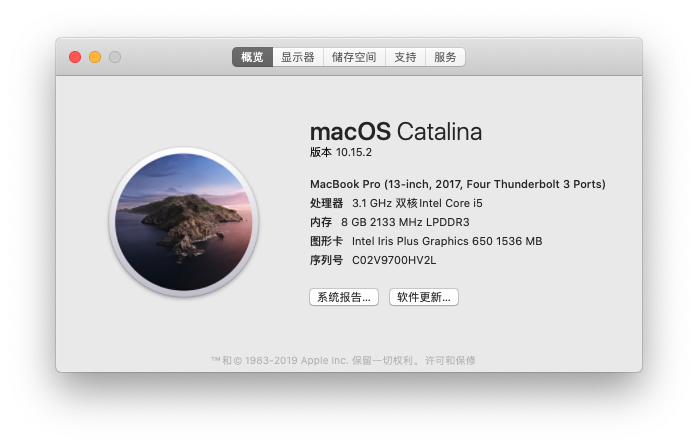
\includegraphics[width=0.8\textwidth]{fig/电脑配置.png}\\
  \caption{电脑配置}
  \label{mre1}
\end{figure}

\begin{lstlisting}[language=bash]
make bench                                                                                           
go test -bench Benchmark -run xx -count 5 -benchmem
goos: darwin
goarch: amd64
pkg: pingcap/talentplan/tidb/mergesort
BenchmarkMergeSort-4    	       1	1120441361 ns/op	134219760 B/op	      10 allocs/op
BenchmarkMergeSort-4    	       1	1171199466 ns/op	134220112 B/op	      12 allocs/op
BenchmarkMergeSort-4    	       1	1169609736 ns/op	134218608 B/op	       7 allocs/op
BenchmarkMergeSort-4    	       1	1316068156 ns/op	134218704 B/op	       8 allocs/op
BenchmarkMergeSort-4    	       1	1444146619 ns/op	134218224 B/op	       6 allocs/op
BenchmarkNormalSort-4   	       1	3878303366 ns/op	      64 B/op	       2 allocs/op
BenchmarkNormalSort-4   	       1	3881277071 ns/op	      64 B/op	       2 allocs/op
BenchmarkNormalSort-4   	       1	3846789734 ns/op	      64 B/op	       2 allocs/op
BenchmarkNormalSort-4   	       1	3880941518 ns/op	      64 B/op	       2 allocs/op
BenchmarkNormalSort-4   	       1	3858949522 ns/op	      64 B/op	       2 allocs/op
PASS
ok  	pingcap/talentplan/tidb/mergesort	30.501s
\end{lstlisting}

\subsection{实现思路}
在编写本次作业的时候,实现了2种归并算法,第一种虽然执行效率高于单线程的快排,但是扩展性不好,代码实现在$badmergesort.go$文件中。于是对第一种方法进行了改进之后
实现了第2种归并算法,代码实现在$mergesort.go$文件中。本节讲解优化后的归并算法实现。

\begin{enumerate}
  \item 基本思路很简单,就是尽量利用机器的cpu资源,将数据根据机器的核数进行划分,每个核分配一组切片数据进行归并排序,每个核对部分数据进行自顶向下的排序之后,得到了和核数相同组数的
  有序切片。
  \item 再使用自底向上的归并排序对这组有序切片进行归并,因为使用自底向上的归并排序可以利用多核资源并行归并。
\end{enumerate}
该归并算法的功能由4个函数实现,分别是MergeSort、merge、coreSort、b2UpMerge。
\subsubsection{MergeSort函数}

MergeSort是算法入口,该函数的功能是根据机器核数对数据进行划分,将数据分发到不同的goroutine上执行,parts记录分组数组在目标数组的下标,因为在后面进行自底向上归并
的时候需要利用分片数组在原始数组的下标值。

\begin{lstlisting}[language=Golang]
  func MergeSort(src []int64) {
    length := len(src)
    numCPU := runtime.NumCPU()

    // 当数组长度小于机器核数的时候,直接使用自带的排序函数排序
    if length < numCPU {
      sort.Slice(src, func(i, j int) bool { return src[i] < src[j] })
      return
    }
  
    interSrc = make([]int64, length)
    parts := make([]partSrc, numCPU)
    batch := length / numCPU

    var wg sync.WaitGroup
    wg.Add(numCPU)
  
    for i := 0; i < numCPU; i++ {
      start := i * batch
      end := start + batch
      if i == numCPU-1 {
        end = length
      }
      parts[i] = partSrc{start, end}
      go func(start, end int) {
        defer wg.Done()
        coreSort(src, start, end)
      }(start, end)
    }
  
    wg.Wait()
    b2UpMerge(src, parts)
  }
\end{lstlisting}

\subsubsection{coreSort和merge函数}
MergeSort函数将数据划分好之后就分配给每个核执行coreSort函数进行排序,这部分的实现就是简单的归并排序算法实现,因为在merge函数中进行归并的时候需要一个辅助数组来暂时存储排序的结果,
为了避免重复初始化中间数组造成gc过多的问题,在MergeSort函数中我们就只初始化了一个和目标数组一样大小的数组用来在merge函数中存储中间数据。
\begin{lstlisting}[language=Golang]
  func merge(src []int64, start, mid, end int) {
    left := start
    right := mid
    idx := start
    for left < mid && right < end {
      if src[left] > src[right] {
        interSrc[idx] = src[right]
        right++
      } else {
        interSrc[idx] = src[left]
        left++
      }
      idx++
    }
  
    for left < mid {
      interSrc[idx] = src[left]
      left++; idx++
    }
  
    for right < end {
      interSrc[idx] = src[right]
      right++; idx++
    }
  
    for i := start; i < end; i++ {
      src[i] = interSrc[i]
    }
  }
  
  func coreSort(src []int64, start, end int) {
    if end-start <= 1 {
      return
    }
    mid := start + (end-start)>>1
    coreSort(src, start, mid)
    coreSort(src, mid, end)
    merge(src, start, mid, end)
  }
\end{lstlisting}

\subsubsection{b2UpMerge 函数}
当每个核分别对属于自己部分的数据排好序之后,使用b2UpMerge对有序切片组进行自底向上的排序,先归并两两有序数组,然后再对归并好的子数组两两归并,因为两两归并的时候数据互不影响,
所以可以并行执行。
\begin{lstlisting}[language=Golang]
  func b2UpMerge(src []int64, parts []partSrc) {
    n := len(parts)
    for size := 1; size < n; size *= 2 {
      var wg sync.WaitGroup
      for low := 0; low < n-size; low += size * 2 {
        start := parts[low].start
        mid := parts[low+size-1].end
        endIdx := low + size*2 - 1
        if endIdx > n-1 {
          endIdx = n - 1
        }
        end := parts[endIdx].end
        wg.Add(1)
        go func(start, mid, end int) {
          defer wg.Done()
          merge(src, start, mid, end)
        }(start, mid, end)
      }
      wg.Wait()
    }
  }
\end{lstlisting}

\subsection{单元测试}
这里对上述函数编写了单元测试,主要是测试b2UpMerge函数在不同CPU核数下的是否能够正确执行,单元测试部分代码在$mergesort\_test.go$文件中。
\begin{lstlisting}[language=Golang]
  func (s *sortTestSuite) TestB2UpMerge(c *check.C) {
    cpus := []int{2, 4, 8, 16, 32, 64, 128}
    lens := []int{1, 3, 5, 7, 11, 13, 17, 19, 23, 29, 1024, 1 << 13, 1 << 17, 1 << 19, 1 << 20}
  
    for i := range lens {
      src := make([]int64, lens[i])
      expect := make([]int64, lens[i])
      for j := range cpus {
        prepare(src)
        copy(expect, src)
        sort.Slice(expect, func(i, j int) bool { return expect[i] < expect[j] })
        numCPU := cpus[j]
        batch := lens[i] / numCPU
        parts := make([]partSrc, numCPU)
        for k := 0; k < numCPU; k++ {
          start := k * batch
          end := start + batch
          if k == numCPU-1 {
            end = lens[i]
          }
          parts[k] = partSrc{start, end}
          srcSlice := src[start:end]
          sort.Slice(srcSlice, func(i, j int) bool { return srcSlice[i] < srcSlice[j] })
        }
        b2UpMerge(src, parts)
        for i := 0; i < len(src); i++ {
          c.Assert(src[i], check.Equals, expect[i])
        }
      }
    }
  }
\end{lstlisting}

\subsection{性能瓶颈分析}
\subsubsection{对初始版本的归并排序进行性能分析}
因为在实现这周作业的时候,刚学习golang,于是在实现第一版归并排序的时候,想尽量使用golang一些特有的用法,结果代码写的一塌糊涂,现在看看都觉得可怕,
这里我们就叫他为BadMergeSort。
\begin{enumerate}
  \item BadMergeSort的实现思路也是一开始根据核数对数据进行划分,当时也没有考虑到gc的问题,没有对数据进行原地排序,而是频繁的创建新的数组,
  使用系统自带的排序算法进行排序。
  \item 而且排好序的数据传递也传递到channel中,总之能用channel的地方全都用到了channel。本以为能加速运算,结果弄巧成拙性能提升很有限。
\end{enumerate}
下面是对这几个归并排序实现进行benchmark的结果(这个是在我笔记本上4核测试的结果),BenchmarkMergeSort代表归并排序的最终的实现,
从测试的结果我们可以看到BadMergeSort每次操作分配内存的次数明显大于其他2种实现。
\begin{lstlisting}[language=bash]
  make bench
  go test -bench Benchmark -run xx -count 5 -benchmem
  goos: darwin
  goarch: amd64
  pkg: pingcap/talentplan/tidb/mergesort
  BenchmarkMergeSort-4      	       1	1138210345 ns/op	134220016 B/op	      11 allocs/op
  BenchmarkMergeSort-4      	       1	1194155018 ns/op	134218992 B/op	       8 allocs/op
  BenchmarkMergeSort-4      	       1	1073539226 ns/op	134218992 B/op	       8 allocs/op
  BenchmarkMergeSort-4      	       1	1239939969 ns/op	134218320 B/op	       7 allocs/op
  BenchmarkMergeSort-4      	       1	1073343467 ns/op	134219376 B/op	       9 allocs/op
  BenchmarkBadMergeSort-4   	       1	17620337709 ns/op	134257976 B/op	      33 allocs/op
  BenchmarkBadMergeSort-4   	       1	18224372022 ns/op	134259544 B/op	      36 allocs/op
  BenchmarkBadMergeSort-4   	       1	17195247246 ns/op	134256824 B/op	      27 allocs/op
  BenchmarkBadMergeSort-4   	       1	17610047098 ns/op	134257688 B/op	      33 allocs/op
  BenchmarkBadMergeSort-4   	       1	18053680387 ns/op	134258072 B/op	      34 allocs/op
  BenchmarkNormalSort-4     	       1	3821154298 ns/op	      64 B/op	       2 allocs/op
  BenchmarkNormalSort-4     	       1	3826700065 ns/op	      64 B/op	       2 allocs/op
  BenchmarkNormalSort-4     	       1	3742681115 ns/op	      64 B/op	       2 allocs/op
  BenchmarkNormalSort-4     	       1	3734559240 ns/op	      64 B/op	       2 allocs/op
  BenchmarkNormalSort-4     	       1	3729463556 ns/op	      64 B/op	       2 allocs/op
  PASS
  ok  	pingcap/talentplan/tidb/mergesort	119.463s
\end{lstlisting}
下面是在16核(Intel(R) Xeon(R) CPU E5620  @ 2.40GHz)的机器上执行benchmark的结果, 虽然是在16核的机器上执行,但是性能几乎没有提升。
\begin{lstlisting}[language=bash]
  make bench
  go test -bench Benchmark -run xx -count 5 -benchmem
  goos: linux
  goarch: amd64
  pkg: pingcap/talentplan/tidb/mergesort
  BenchmarkMergeSort-16       	       1	1001018177 ns/op	134245904 B/op	      79 allocs/op
  BenchmarkMergeSort-16       	       1	1137368279 ns/op	134227152 B/op	      29 allocs/op
  BenchmarkMergeSort-16       	       1	1057554398 ns/op	134224624 B/op	      29 allocs/op
  BenchmarkMergeSort-16       	       1	1027310401 ns/op	134224336 B/op	      30 allocs/op
  BenchmarkMergeSort-16       	       1	1068874930 ns/op	134222896 B/op	      27 allocs/op
  BenchmarkBadMergeSort-16    	       1	46920872854 ns/op	134393560 B/op	     167 allocs/op
  BenchmarkBadMergeSort-16    	       1	48372915392 ns/op	134392440 B/op	     161 allocs/op
  BenchmarkBadMergeSort-16    	       1	48121852679 ns/op	134376152 B/op	     102 allocs/op
  BenchmarkBadMergeSort-16    	       1	46876084335 ns/op	134391896 B/op	     155 allocs/op
  BenchmarkBadMergeSort-16    	       1	45784126502 ns/op	134389944 B/op	     135 allocs/op
  BenchmarkNormalSort-16      	       1	5618693108 ns/op	      64 B/op	       2 allocs/op
  BenchmarkNormalSort-16      	       1	5616926535 ns/op	      64 B/op	       2 allocs/op
  BenchmarkNormalSort-16      	       1	5622215662 ns/op	      64 B/op	       2 allocs/op
  BenchmarkNormalSort-16      	       1	5658672791 ns/op	      64 B/op	       2 allocs/op
  BenchmarkNormalSort-16      	       1	5616231879 ns/op	      64 B/op	       2 allocs/op
  PASS
  ok  	pingcap/talentplan/tidb/mergesort	282.609s
\end{lstlisting}

关于BadMergeSort的实现就不多说了,下面看一下乱用channel的结果,从火焰图可以看到大部分cpu时间都耗在了golang的协程切换中,
尤其是$runtime.pthread\_cond\_wait$和$runtime.pthread\_cond\_signal$两个函数上,因为协程在遇到管道读写时条件无法满足,当前协程会被阻塞,
runtime便会调用该mcall放弃当前协程并执行一次协程调度,在BadMergeSort的实现中,尤其是两个有序数组归并部分也是用了channel来实现,造成了
大量的时间耗费在协程调度和管道等待中。

\begin{lstlisting}[language=bash]
  go tool pprof cpu.prof                                                                                                      
  Type: cpu
  Time: Jan 4, 2020 at 4:41pm (CST)
  Duration: 1.54mins, Total samples = 2.45mins (158.94%)
  Entering interactive mode (type "help" for commands, "o" for options)
  (pprof) top
  Showing nodes accounting for 2.23mins, 91.10% of 2.45mins total
  Dropped 85 nodes (cum <= 0.01mins)
  Showing top 10 nodes out of 55
        flat  flat%   sum%        cum   cum%
    0.99mins 40.53% 40.53%   0.99mins 40.55%  runtime.pthread_cond_wait
    0.40mins 16.23% 56.77%   0.40mins 16.24%  runtime.pthread_cond_signal
    0.29mins 11.73% 68.50%   0.29mins 11.73%  runtime.usleep
    0.24mins  9.82% 78.32%   0.24mins  9.82%  runtime.(*waitq).dequeue
    0.15mins  6.02% 84.34%   0.25mins 10.25%  sort.doPivot_func
    0.08mins  3.46% 87.80%   0.08mins  3.46%  pingcap/talentplan/tidb/mergesort.BadMergeSort.func1.1
    0.03mins  1.05% 88.85%   0.03mins  1.05%  internal/reflectlite.Swapper.func5
    0.02mins  0.99% 89.84%   0.02mins  0.99%  runtime.newstack
    0.02mins  0.67% 90.50%   0.02mins  0.67%  runtime.casgstatus
    0.01mins   0.6% 91.10%   0.07mins  2.86%  runtime.lock
\end{lstlisting}

\begin{figure}[H]
  \centering
  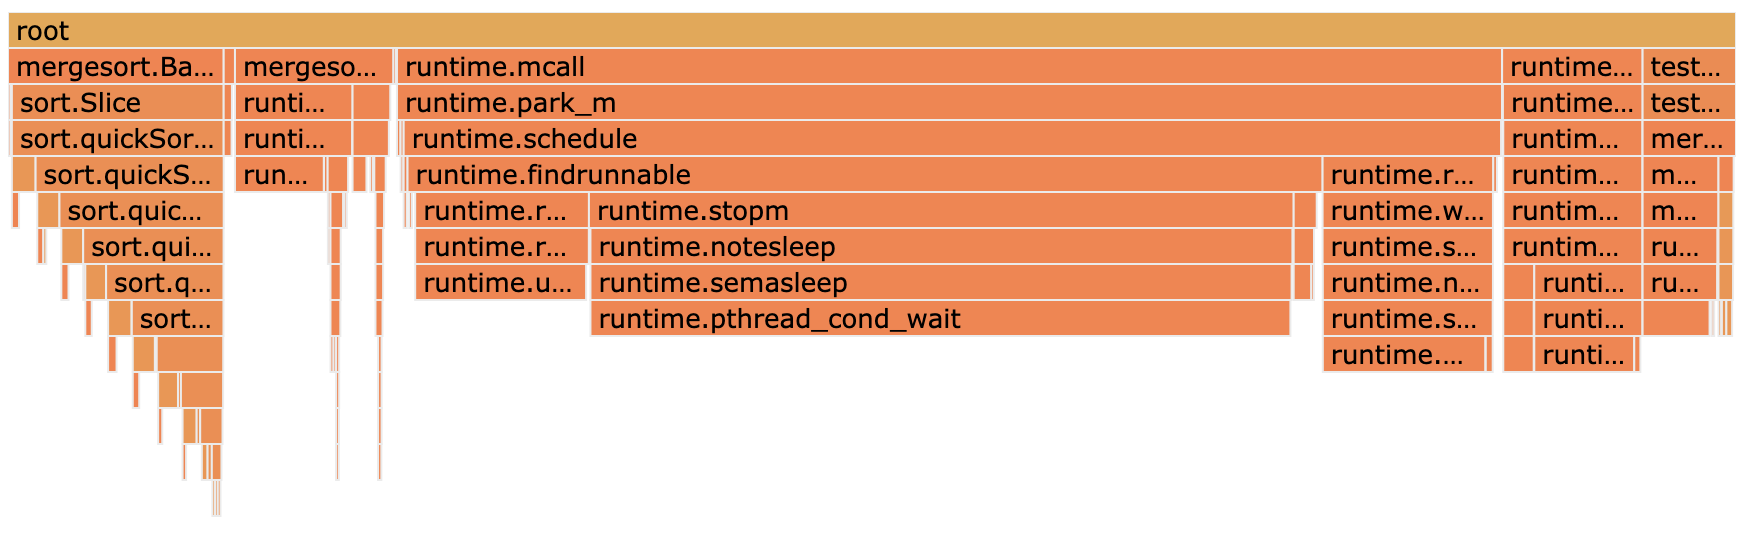
\includegraphics[width=0.8\textwidth]{fig/bad-cpu.png}\\
  \caption{BadMergeSort-CPU-火焰图}
  \label{mre1}
\end{figure}

\subsubsection{对优化后的归并排序进行性能分析}
优化后的归并算法,去掉了channel的使用,减少了不必要的内存分配,具体的优化在2.1实现思路上写了,所以这里就不赘述了。
下面对优化后的归并排序进行分析,从结果上明显看到大部分的cpu时间耗费在merge运算上,从火焰图上也能看出没有了runtime的耗时,而且也没有gc相关函数的执行,所以就不进行
mem分析了。
\begin{lstlisting}[language=bash]
  go tool pprof cpu.prof                                                                                                      
  Type: cpu
  Time: Jan 4, 2020 at 7:05pm (CST)
  Duration: 13.05s, Total samples = 17.23s (132.05%)
  Entering interactive mode (type "help" for commands, "o" for options)
  (pprof) top
  Showing nodes accounting for 17s, 98.67% of 17.23s total
  Dropped 37 nodes (cum <= 0.09s)
  Showing top 10 nodes out of 23
        flat  flat%   sum%        cum   cum%
      13.90s 80.67% 80.67%     13.90s 80.67%  pingcap/talentplan/tidb/mergesort.merge
       0.76s  4.41% 85.08%     13.93s 80.85%  pingcap/talentplan/tidb/mergesort.coreSort
       0.55s  3.19% 88.28%      0.55s  3.19%  runtime.newstack
       0.54s  3.13% 91.41%      0.54s  3.13%  sync.(*Mutex).Unlock
       0.48s  2.79% 94.20%      0.48s  2.79%  sync.(*Mutex).Lock
       0.46s  2.67% 96.87%      0.46s  2.67%  runtime.memclrNoHeapPointers
       0.17s  0.99% 97.85%      1.36s  7.89%  math/rand.(*lockedSource).Int63
       0.08s  0.46% 98.32%      1.45s  8.42%  pingcap/talentplan/tidb/mergesort.prepare
       0.05s  0.29% 98.61%      0.13s  0.75%  math/rand.(*rngSource).Int63
       0.01s 0.058% 98.67%      1.37s  7.95%  math/rand.(*Rand).Int63
\end{lstlisting}

\begin{figure}[H]
  \centering
  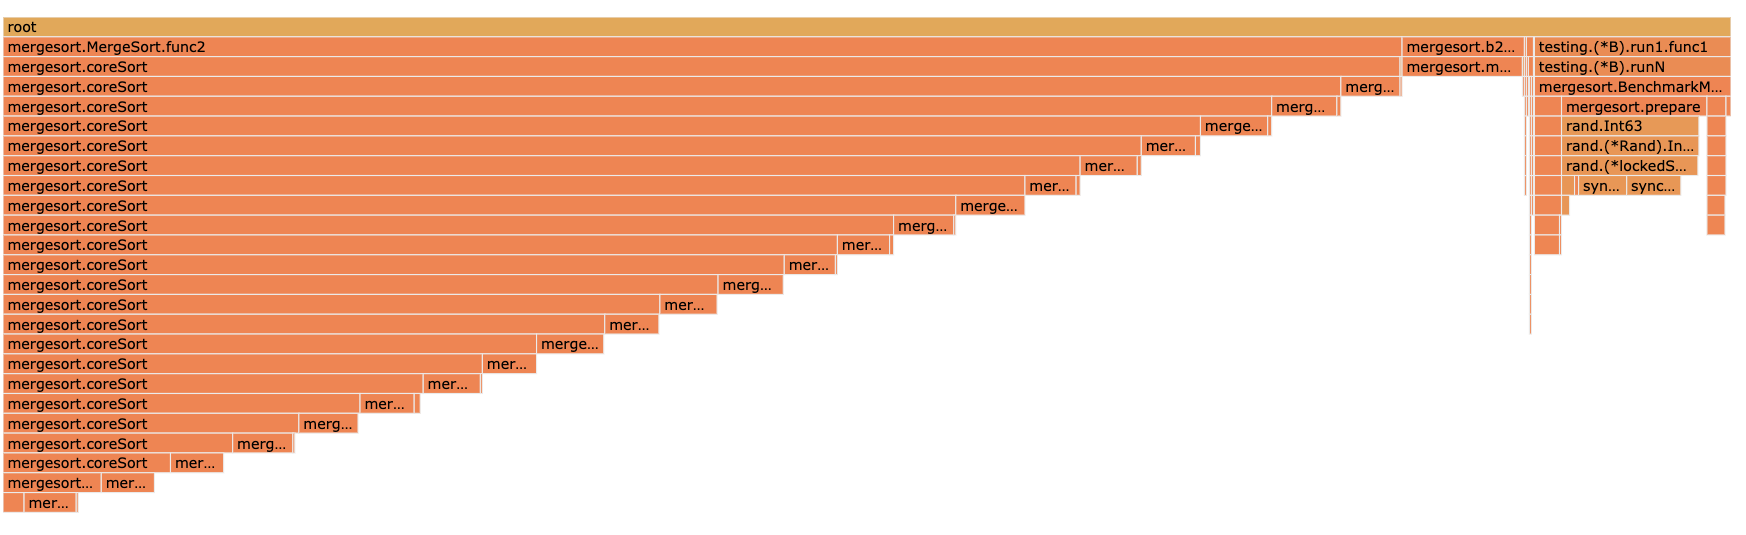
\includegraphics[width=0.8\textwidth]{fig/cpu.png}\\
  \caption{MergeSort-CPU-火焰图}
  \label{mre1}
\end{figure}
\end{document}